\title{Ubiquitous techniques in Hodge theory}
\author{\textit{Based on a lecture series by }Inder Kaur.}
\date{December 2023}
\maketitle

\newcommand{\Jac}{\mathop{\mathcal{J\kern -0.5pt a\kern -0.5pt c\kern -1pt}}}
\newcommand{\IJac}{\mathop{I\mathcal{J\kern -0.5pt a\kern -0.5pt c\kern -1pt}}}
\newcommand{\Moduli}{\ensuremath{\mathscr{M}}}

The classical Torelli theorem is a celebrated result that shows smooth complex
curves are determined by their Jacobians (i.e.\ the moduli of line bundles). One
can ask if a similar statement holds for moduli spaces of rank \(2\) bundles,
and a positive answer was provided by Mumford and Newstead, who showed that
a smooth projective curve can be recovered from any moduli space of rank \(n\)
stable bundles (with degree coprime to \(n\)). Further, one may ask about
singular curves-- this is a much harder question which was only recently
answered by Kaur et al. Underlying such results are powerful techniques from
Hodge theory which reduce algebro-geometric problems to linear algebra and the
study of tori.

\subsection{About} This course on Hodge theory was a part of a Winter School
for early career researchers, organised by the UK Algebraic
Geometry Network. The lectures were delivered in-person in
the University of Warwick, and were transcribed by Parth Shimpi. These
notes have undergone several amendments and are not a verbatim recall of
the lectures, therefore discretion is advised when using this material. The
notes are available online at
\url{https://pas201.user.srcf.net/documents/2023-ukag-hodge-theory.pdf}. 

All
errors and corrections should be communicated to by email to
\url{pas201@srcf.net}.

\subsection{Supplement on complex tori} The lectures assume some familiarity
with Abelian varieties, in particular the Appell-Humbert correspondence and the
notion of theta divisors shows up. A short introduction to the theory can be found at \url{https://pas201.user.srcf.net/documents/2023-complex-tori.pdf}.

\section{Hodge decomposition}
We have developed various cohomology theories on complex varieties-- most
notably the de Rham cohomology and sheaf cohomology. One can ask if, for a
smooth variety \(X\), there is a relation between the two?

\subsection{The Dolbeault cohomology groups}
Recall that if \(F\) is a sheaf on a smooth \(n\)-dimensional complex manifold
\(X\), then to compute the sheaf cohomology groups \(\HH^k(X,F)\) we need an
acyclic resolution of \(F\). This is given by a complex of sheaves \(F^\bullet =
(F^0\to F^1\to F^2\to ...)\) such that for any \(i\geq 0\),
\(\HH^{>0}(X,F^i)=0\) (i.e.\ the \(F^i\) are \textit{acyclic}) and there is an
injective morphism \(F\to F^0\) such that the complex \(0\to F \to F^\bullet\)
is exact. The cohomology groups \(\HH^k(X,F)\) are by definition the cohomologies of the complex \(0\to F^0(X)\to F^1(X)\to F^2(X)\to... \) obtained by applying the global sections functor to \(F^\bullet\).

Now the sheaf of holomorphic \(p\)-forms \(\Omega^p_X\) is the \(p\)th exterior
power of the cotangent bundle. What is \(\HH^q(X,\Omega_X^p)\)? We need an
acyclic resolution as above. Choosing local complex coordinates \(z_1,...,z_n\)
on an open set \(U\), we can consider the spaces of smooth complex \((p,q)\)-forms
\[A^{p,q}(U)=\left\{\sum f_{IJ}dz_I\wedge d\bar{z}_J\;\middle|\; |I|=p,\; |J|=q\right\}\]
which together give a sheaf \(A^{p,q}\) of smooth \((p,q)\)-forms on \(X\). Each
\(A^{p,q}\) can be shown to be acyclic using \v{C}ech covers and partitions of
unity, and there is a natural injection \(\Omega^p\into A^{p,0}\). Moreover, sheaves \(A^{p,q}\) come equipped with the differential
\(\bar\partial:A^{p,q}\to A^{p,q+1}\) given locally by \[\bar\partial \left(\sum f_{IJ}dz_I\wedge
d\bar{z}_J\right) = \sum \sum \frac{\partial f_{IJ}}{\partial \bar{z}_j} d
\bar{z}_j\wedge dz_I \wedge d\bar{z}_J,\] and by the
\(\bar\partial\)--Poincar\'e lemma the complex of sheaves
\(0\to \Omega^p_X\to A^{p,\bullet}\) is exact. Thus we can use this acyclic resolution to compute the sheaf cohomology
\(\HH^{p,q}(X)\coloneq \HH^q(X,\Omega^p_X).\)

If \(X\) is compact and connected, the famous Hodge theorem asserts that each
class in \(\HH^{p,q}(X)\) can be represented by a unique harmonic\footnote{With
respect to the Laplacian \(\Delta=\bar\partial \bar\partial^\ast - \bar\partial^
\ast \bar\partial\).} \((p,q)\)-form, and the space \(\HH^{p,q}(X)\) (hence equal to the space of Harmonic \((p,q)\)-forms) is finite dimensional. The \textit{Hodge numbers} are defined as the dimensions \(\text{h}^{p,q}(X)=\dim \HH^{p,q}(X)\).

\begin{exercise}
    Show that \(\text{h}^{p,q}(X)=\text{h}^{n-p,n-q}(X)\) for
    \(n=\dim X\). [Hint: Serre duality.]
\end{exercise}

\subsection{The Hodge decomposition theorem} In general, the Dolbeault
cohomology and the de Rham cohomology aren't strongly related and the two
associated Laplacians \((\bar\partial\bar\partial^\ast - \bar\partial^\ast
\bar\partial),(dd^\ast-d^\ast d)\) are independent. However, when \(X\) is
a compact manifold with a K\"ahler metric (e.g.\ if \(X\) is projective), then
the two associated Laplace operators are equal up to scaling. Thus the de Rham
cohomology \(\HH^k(X,\mathbb{C})\), equal to the space of harmonic \(k\)-forms,
decomposes into the Dolbeault cohomology groups \(\HH^{p,q}(X)\) and we obtain
the following result which gives a definitive relation between the de Rham
cohomology and sheaf cohomology on \(X\).

\begin{theorem}[(Hodge decomposition)]
    Let \(X\) be a smooth \(n\)-dimensional compact complex manifold that admits
    a K\"ahler metric. Then for \(k\leq n\), we have a decomposition of
    cohomology groups \(\HH^k(X,\mathbb{C})
    =\bigoplus_{p+q=k}\HH^{p,q}(X)\) and moreover, the decomposition obeys a
    \textit{Hodge symmetry} \(\overline{\HH^{p,q}(X)}=\HH^{q,p}(X)\).
\end{theorem}

By Hodge symmetry, we have \(\text{h}^{p,q}=\text{h}^{q,p}(X)\) and by the Hodge
decomposition, we can compute the Betti numbers as \(b_k(X)=\sum_{p+q=k}
\text{h}^{p,q}(X)\). This data of Hodge numbers is usually packaged in a
\textit{Hodge diamond} of the form below.
\[\begin{tikzcd}[column sep=0em, row sep = 0em]
    &&&&\hh^{0,0}&&&& \\
    &&&\hh^{1,0} && \hh^{0,1} &&&\\
    &&\hh^{2,0}&&\hh^{1,1} && \text{h}^{0,2} && \\
    \hh^{n,0} &&&&\vdots&&&&\hh^{0,n} \\
    &&&&\phantom{h}&&&& \\
    &&&\hh^{n,n-1} && \hh^{n-1,n} &&& \\\\
    &&&&\hh^{n,n}&&&&
\end{tikzcd} \]
Then Hodge symmetry says the diamond is symmetric about the vertical axis, while
Serre duality says it is symmetric about the midpoint. The Hodge decomposition
theorem gives some observations-- for instance if \(k\) is odd then \(\dim
\HH^{k}(X,\mathbb{C})\) is even. Secondly, \(\dim \HH^0(X,\Omega^p_X) = \dim
\HH^p(X,\mathscr{O}_X)\).

\begin{example}
    If \(X\) is a smooth complex curve of genus \(g\), then
    \(\text{b}_1(X)=2g\) and hence \(\text{h}^{1,0}=\text{h}^{0,1}=g\).
\end{example}

\begin{exercise}
    Compute the Hodge diamond of a K3 surface. [Hint: all K3 surfaces are
    diffeomorphic with trivial \(\text{b}_1\) and Euler characteristic \(24\).]
\end{exercise}

\begin{exercise}
    Are the Hodge numbers birationally invariant? [Hint: check for the blow-up
    of a surface.]
\end{exercise}

\subsection{Pure Hodge structures} As is often the case in mathematics, we are
more interested in the phenomenon of decomposition than the actual numbers.
Hence we make the following abstraction.

\begin{definition}
    A \textit{pure \(\mathbb{Z}\)-Hodge structure of weight \(k\)} is given by a
    finitely generated Abelian group \(V_\mathbb{Z}\) and a decomposition
    \(V_\mathbb{C}\coloneq V_\mathbb{Z}\otimes \mathbb{C}=\bigoplus_{p+q=k}
    V^{p,q}\) such that \(\overline{V^{p,q}}=V^{q,p}\).
\end{definition}

The data of a pure \(\mathbb{Z}\)-Hodge structure of weight \(k\) on
\(V_\mathbb{Z}\) is equivalent to the data of a filtration
\(V_\mathbb{C}=F^0\supset ... \supset F^k\) with
\(V_\mathbb{C}=F^p\oplus \overline{F^{k-p+1}}\) for all \(p\). Indeed in this
case we have \(V^{p,q}=F^p\cap \overline{F^q}\) and given the \(V^{p,q}\)s we
can recover the filtration as \(F^p=\bigoplus_{p'\geq p}V^{p',k-p'}\).

\begin{remark}
    Note that \(\mathbb{C}\)-vector spaces do not have an intrinsic notion of
    complex conjugation. However, for a chosen basis this makes sense, and
    \(V_\mathbb{C}\) has a canonical choice of basis coming from
    \(V_\mathbb{Z}\).
\end{remark}

\begin{definition}
Let \((V_\mathbb{Z},V^{p,q})\) and \((W_\mathbb{Z},W^{p,q})\) denote two pure
\(\mathbb{Z}\)-Hodge structures of weights \(k\), \(k+2r\) respectively. A
bidegree \((r,r)\) morphism of Hodge structures is given by a linear map
\(\varphi:V_\mathbb{Z}\to W_\mathbb{Z}\) such that \(\varphi(V^{p,q})\subset
W^{p+r,q+r}\) (or equivalently, \(\varphi (F^pV_\mathbb{C})\subset
F^{p+r}W_\mathbb{C})\).
\end{definition}

\begin{example}
    Let \(f:X\to Y\) be a morphism between smooth projective complex varieties
    of dimensions \(n, n+r\) respectively. By the Hodge decomposition theorem,
    the integral cohomology groups \(\HH^k(X,\mathbb{Z})\) have a pure Hodge
    structure of weight \(k\). Then the map \(f^\ast:\HH^k(Y,\mathbb{Z})\to
    \HH^k(X,\mathbb{Z})\) is a bidegree \((0,0)\) morphism of Hodge structures.
    On the other hand, the Gysin morphism \(f_\ast:\HH^k(X,\mathbb{Z})\to
    \HH^{k+2r}(Y,\mathbb{Z})\) (i.e.\ the pushforward \(f_\ast :
    \HH_{2n-k}(X,\mathbb{Z})\to \HH_{2n-k}(Y,\mathbb{Z})\) composed with
    Poincar\'e duality) is a morphism of bidegree \((r,r)\).
\end{example}

\subsection{Intermediate Jacobians} Given a Hodge structure, one can sometimes
naturally construct a complex torus out of it. To see this, fix a lattice
\(V_\mathbb{Z}\) of rank \(2r\), and a pure \(\mathbb{Z}\)-Hodge structure
\(V^{p,q}\) of weight \(2k-1\) on it. Then \(V_\mathbb{C}/F^k = \overline{F^k}=
V^{0,2k-1}\oplus ... \oplus V^{k-1,k}\) is an \(r\)-dimensional
\(\mathbb{C}\)-vector space, and \(V_\mathbb{Z}\) forms a lattice inside it via
the natural inclusion \(V_\mathbb{Z}\into V_\mathbb{C}\onto \overline{F^k}\).
(Indeed, the only thing to check is that \(V_\mathbb{Z}\cap F^k=0\), but this is
true since \(V_\mathbb{Z}\) is invariant under conjugation.) Thus
\(V_\mathbb{C}/(F^k\oplus V_\mathbb{Z})\) is an \(r\)-dimensional complex torus,
called the \textit{intermediate Jacobian} associated to the Hodge structure. The
\textit{period} of this torus is \(V_\mathbb{Z}\).

\begin{definition}
    Given a pure Hodge structure \((V_\mathbb{Z}, V^{p,q})\) of weight \(k\), a
    \textit{polarisation} is a non-degenerate bilinear form
    \(Q:V_\mathbb{Z}\times V_\mathbb{Z}\to \mathbb{Z}\) satisfying the
    Hodge--Riemann relations
    \begin{enumerate}[(i)]
        \item \(Q(v,w)=(-1)^k Q(w,v)\) for all \(v,w\in V_\mathbb{Z}\),
        \item \(Q(v,w)=0\) for all \(v\in V^{p,q}\), \(w\in
            V^{p',q'}\) whenever \(p\neq q'\), and
        \item \((-1)^\frac{k(k-1)}{2}i^{p-q} Q(v,\bar v)>0\) for \(v \in
            V^{p,q}\setminus 0\).
    \end{enumerate}
\end{definition}

One checks that this definition is such that whenever the Hodge structure has
odd weight (consequently \(V_\mathbb{Z}\) has even rank), the polarisation of
the Hodge structure is also a polarisation on the intermediate Jacobian (i.e.\ a
positive definite Hermitian form \(H:\overline{F}_k\times \overline{F}_k\to
\mathbb{C}\) that is integral on \(V_\mathbb{Z}\) and satisfies the Riemann
period relation \(\text{Im}H(iv,iw)=\text{Im}H(v,w)\).) Thus intermediate
Jacobians of polarised Hodge structures (whenever defined) are polarised Abelian
varieties.

\begin{example}
    If \(X\) is an \(n\)-dimensional  K\"ahler manifold with fixed K\"ahler
    class \(\omega\in \HH^{1,1}(X)\), then the intersection form on
    \(\HH^k(X,\mathbb{Z})\) given by \((\alpha,\beta)\mapsto
    \int_{[X]}\omega^{n-k}\wedge \alpha\wedge \beta\) is a polarisation. For
    \(k>0\), the \textit{\(k\)th intermediate Jacobian} of \(X\) is thus an
    Abelian variety given by
    \[
       \IJac^k X \coloneq
       \frac{\HH^{2k-1}(X,\mathbb{C})}{F^k\HH^{2k-1}(X,\mathbb{C})\oplus
       \HH^{2k-1}(X,\mathbb{Z})}.
    \]
\end{example}

The first intermediate Jacobian is simply called the \textit{Jacobian} of \(X\),
given by \(\Jac X\coloneq \HH^{1}(X,\mathscr{O}_X)/\HH^1(X,\mathbb{Z})\).

Intermediate Jacobians are Hodge--theoretic invariants of a smooth variety that
often determine its geometry. For example, [Clemens--Griffiths] show that if
\(X\) is a smooth projective 3-fold with \(\HH^{0,3}(X)=0\) (e.g.\ if \(X\) is
Fano) then \(X\) is rational only if \(\IJac^2X\) decomposes into a product
\(\IJac^1C_1\times ... \times \IJac^1C_n\) for smooth curves \(C_1,...,C_n\).
On the other hand, they also compute that if \(X\) arises as a cubic
hypersurface in \(\mathbb{P}^4\) then \(\IJac^2X\) is five dimensional and
principally polarised. In particular there is a well-defined theta divisor up to
translation, which has a single isolated singularity. Since the theta divisor
for products of the form \(\IJac^1C_1\times ... \times \IJac^1C_n\) cannot have
isolated singularities, this shows that a general cubic 3-fold is irrational.

\section{Torelli and Mumford--Newstead theorems}

When is a complex manifold determined by its Hodge theory?

\begin{exercise}
    Exhibit two non-isomorphic projective varieties with isomorphic Hodge
    structures.
\end{exercise}

Hence just looking at the Hodge structure does not suffice. However, it was
shown by Torelli that for a smooth curve \(X\) it is sufficient to check the
polarised Hodge structure on \(\HH^1(X,\mathbb{Z})\). Recall if \(X\) has genus
\(g\), then \(\HH^1(X,\mathbb{Z})\) has a pure Hodge structure of weight \(1\).
The cup product on cohomology \(Q(\alpha,\beta)=\int_{[X]}\alpha \wedge \beta\)
gives a polarisation, which can be explicitly described by choosing a basis
\(\alpha_1,...,\alpha_g,\beta_1,...,\beta_g\) for the lattice
\(\HH^1(X,\mathbb{Z})\). We then have
\(Q(\alpha_i,\alpha_j)=Q(\beta_i,\beta_j)=0\) for all \(i, j\) and
\(Q(\alpha_i,\beta_j)=\delta_{ij}\). In other words, \(Q\) is given by the
\(2g\times 2g\) matrix \(\left[\begin{smallmatrix} 0 & \text{Id} \\
-\text{Id} & 0 \end{smallmatrix}\right]\).

It follows that the Jacobian \(\Jac(X)\) is principally polarised, with a
well-defined theta divisor.

\begin{theorem}[(Torelli)]
    Two smooth curves \(X,Y\) are isomorphic if and only if there is an isometry
    of polarised Hodge structures \(\HH^1(X,\mathbb{Z})\to
    \HH^2(Y,\mathbb{Z})\). Equivalently, if there is an isomorphism \(\Jac X
    \cong \Jac Y\) that restricts to an isomorphism of theta divisors.
\end{theorem}

\subsection{Jacobians as moduli spaces} Let \(X\) be a smooth projective
variety. There is an associated algebro-geometric construction called the
\textit{Picard variety} \(\Pic^0(X)\), which is a moduli space of line bundles
on \(X\) with trivial Chern class. This is constructed as follows-- write
\(\mathscr{O}_X^\times\) for the sheaf of nowhere--vanishing holomorphic
functions on \(X\), and recall that \(\Pic X = \HH^1(X,\mathscr{O}_X^\times)\)
is the group of line bundles on \(X\) up to isomorphism. Considering the
\textit{exponential exact sequence} \(0\to \mathbb{Z}\xrightarrow{\;2\pi
i\;}\mathscr{O}_X\xrightarrow{\;\exp\;} \mathscr{O}_X^\times \to 0\), the
associated long exact sequence is given by
\[\to
\HH^0(X,\mathscr{O}_X)\xrightarrow{\;\exp\;}\HH^0(X,\mathscr{O}_X^\times)
\to \HH^1(X,\mathbb{Z})\xrightarrow{j} \HH^1(X,\mathscr{O}_X)\to
\underbrace{\HH^1(X,\mathscr{O}_X^\times)}_{\text{Pic}X}\xrightarrow{\;c_1\;}
\HH^2(X,\mathbb{Z})\to \HH^2(X,\mathscr{O}_X)\to\]
and the \textit{first Chern map} \(c_1\) is by definition the coboundary
map shown. By definition, \(\Pic^0(X)=\ker c_1\).

Now \(X\) is compact so \(\exp:\mathbb{C}\to \mathbb{C}^\times\) is
surjective, and hence \(j\) is injective, in fact it is the natural map
\(\HH^1(X,\mathbb{Z})\into \HH^1(X,\mathbb{C})\onto \HH^{1,0}(X)\). Chasing
through the exact sequence, we have
\(\Pic^0(X)=\HH^1(X,\mathscr{O}_X)/\HH^1(X,\mathbb{Z})\) which we recognise as
the Jacobian \(\Jac X\). Hence line bundles on a smooth projective varieties
are determined by their Chern class and an element of the Jacobian \(\Jac X\).

\begin{exercise}
    Show that simply connected projective varieties have trivial Jacobians.
\end{exercise}

If \(X\) is a connected curve, then \(\HH^2(X,\mathscr{O}_X)=0\) and hence
\(c_1\) is surjective (given by the degree map). Thus \(\text{Pic}^0X\)
parametrises line bundles of degree zero, and is called the \textit{Jacobian}.
This is a classical construction going back to Riemann.

\begin{remark}
    Here is how Riemann (allegedly) showed \(\Jac X\) is the parameter space of
    degree zero line bundles. For curves there is an identification
    \(\HH^{0,1}(X)\cong \Hom(\HH^{1,0}(X),\mathbb{C})\), and Riemann computed
    the map \(j\) by taking a cycle \([Z]\in \HH^1(X,\mathbb{Z})\), and mapping
    it to the functional \(\omega\mapsto \int_Z \omega\) on the space of
    holomorphic \(1\)-forms \(\HH^{1,0}(X)\). This is called the \textit{period
    map}, since it identifies \(\HH^1(X,\mathbb{Z})\) with the period lattice of
    the Jacobian.

    Continuing this analytic picture, fix a base point \(p_0\in X\) and choose
    paths connecting it to every other point in \(X\). Integration along these
    chosen paths gives a morphism \(X\to \HH^{0,1}(X)\) by mapping \(p\in X\) to
    the functional \(\omega\mapsto \int_{p_0}^p\omega\). The induced map \(X\to
    \Jac X\) is independent of the choice of paths, and extends linearly to a
    well-defined map from degree zero divisors on \(X\) called the
    \textit{Abel--Jacobi morphism}. Riemann showed that the kernel of this map
    \(\text{Div}^0(X)\to \Jac X\) is precisely the group of principal divisors,
    giving an isomorphism \(\Pic^0(X)\cong \Jac X\).
\end{remark}

More generally, we use the term Abel--Jacobi map to refer to any map
induced from the map \(X\to \Pic^0(X)\) sending \(p\in X\) to the line bundle
\(\mathscr{O}(p-p_0)\) for a fixed base point \(p_0\in X\). In particular, we
talk of the \(d\)th Abel Jacobi map \(X^{(d)}\to \Pic^0X\) which sends a tuple
\((p_1,...,p_d)\) in the symmetric power \(X^{(d)}\) to the line bundle
\(\mathscr{O}(p_1+...+p_d-d\cdot p_0)\).

\subsection{Theta divisors of Jacobians} Recall that if \(X\) is a smooth curve
then the intersection pairing on \(\HH^1(X,\mathbb{Z})\) has determinant \(1\),
and hence the polarisation on \(\Jac X\) is principal. This gives an ample line
bundle with a unique global section (up to scaling), and the associated divisor
of zeros of this bundle is called the theta divisor. This is well understood.

\begin{theorem}
    Let \(X\) be a smooth projective curve of genus \(g\geq 1\) and choose a base
    point \(p_0\in X\). Then the Abel--Jacobi map \(X^{(g-1)}\to \Pic^0X\) is
    birational and surjective onto the theta divisor.
\end{theorem}

Thus identifying \(\Pic^0(X)\) with the space \(\Pic^d(X)\) of degree \(d\)
line bundles, we see that the theta divisor is precisely the locus where
\(\HH^0(X,-)\) does not vanish. It can be shown that this has singular locus of
dimension \(g-3\) when \(X\) is hyperelliptic, and \(g-4\) otherwise. In
particular, products of Jacobians of curves never have isolated singularities--
this is an essential step in Clemens--Griffiths' proof of the irrationality of
cubic 3-folds.


\subsection{The Mumford--Newstead theorem} The construction of the Jacobian and
the Torelli theorem predate Hodge theory. However, these tools become
indispensable when generalising the results-- for instance, one can ask if the
curve also determined by the moduli space \(\Moduli_{2,d}X\) of stable vector
bundles of rank \(r=2\) and odd degree \(d\) (this condition ensures semistable
bundles are stable and the moduli space is smooth). A positive answer is
provided by [Mumford--Newstead], who show that \(X\) can be recovered from the
second intermediate Jacobian \(\IJac^2(\Moduli_{2,d}X)\).

We briefly discuss the construction. The moduli space
\(\Moduli_{2,d}(X)\) is a smooth projective complex variety of dimension
\(3g-3\) (in general, the dimension is \((r^2-1)(g-1)\)). The moduli space is also unirational, i.e.\ there is a dominant morphism
\(\mathbb{P}^{3g-3}\dashrightarrow\Moduli_{2,d}(X)\). In particular there are no
global regular \(p\)-forms for \(p\geq 1\), and we have
\(\hh^{p,0}=\hh^{0,p}=0\). It follows that the second intermediate Jacobian is
simply
\[\IJac^2(\Moduli_{2,d}X)=\frac{\HH^{1,2}(\Moduli_{2,d}X)}{\HH^3(\Moduli_{2,d}X,\mathbb{Z})}.\]
Mumford and Newstead compute the cohomology group
\(\HH^3(\Moduli_{2,d}X,\mathbb{Q})\) as having \(2g+2\) generators. Of
these, two come from the universal family on the moduli space and the remaining
\(2g\) form a group isomorphic to \(\HH^1(X,\mathbb{Z})\). We have the following.

\begin{theorem}[(Mumford--Newstead)]
    There is a Hodge isometry \(\psi:\HH^1(X,\mathbb{Z})\to
    \HH^3(\Moduli_{2,d}X,\mathbb{Z})\) that induces an isomorphism
    \(\Jac X\cong \IJac^2(\Moduli_{2,d}X)\) preserving theta divisors. In
    particular, a smooth projective curve is uniquely determined by the moduli
    space of rank \(2\) bundles of a fixed odd--degree determinant.
\end{theorem}

More generally, a similar result holds for the moduli spaces of stable vector
bundles with fixed co-prime rank and degree.

\section{Nodal curves and mixed Hodge structures}

What happens if \(X\) is an irreducible nodal curve with one node? Using
classical techniques (i.e.\ without invoking Hodge theory), the following
analogue of the Torelli theorem can be shown.

\begin{theorem}[(Namikawa)]
    If \(X,X'\) are two irreducible nodal curves such that their normalisations
    are not hyper-elliptic and have genus \(g\geq 4\), then \(X\cong X'\) if and
    only if \(\Jac X\cong \Jac X'\).
\end{theorem}

To obtain a version of the Mumford--Newstead theorem, we need some form of Hodge
theory on singular varieties. But for an irreducible nodal curve of genus \(g\),
we see that the rank of \(\HH^1(X,\mathbb{Z})=\mathbb{Z}^{2g+1}\) is odd and
hence there are no pure Hodge structures. To remedy this, we make the following
definition.

\begin{definition}
    A \textit{mixed \(\mathbb{Z}\)-Hodge structure} is given by a finite
    rank \(\mathbb{Z}\)-module \(V_\mathbb{Z}\), equipped with an
    increasing \textit{weight filtration} \(0=W_0\subset W_1\subset...\subset
    W_n=V_\mathbb{Q}\) and a decreasing \textit{Hodge filtration}
    \(V_\mathbb{C}=F^0\supset F^1\supset F^2\supset ...\) such that the induced
    filtration on each graded piece \(\text{Gr}_kW^\bullet=W_k/W_{k-1}\) is a
    pure \(\mathbb{Z}\)-Hodge structure.
\end{definition}

\begin{example}
    A mixed Hodge structure with trivial weight filtration is precisely a pure
    Hodge structure.
\end{example}

\begin{example}[Normalisation of a nodal curve]
    Let \(X\) be an irreducible curve with a node at \(p\in X\), and
    \(\pi:\tilde X \to X\) be its normalisation i.e.\ \(\tilde X\) is a smooth
    genus \(g\) curve and \(\pi\) identifies the two points \(q_0,q_1\in\tilde
    X\) in the exceptional fiber and is an isomorphism elsewhere. It follows
    that there is a short exact sequence of singular cochain-complexes
    \(0\to C^\bullet(X,\mathbb{Q})\to C^\bullet(\tilde X,\mathbb{Q})\to
    C^\bullet(\{p\},\mathbb{Q})\to 0\), and an associated long exact sequence
    which computes \(\HH^1(X,\mathbb{Q})=\HH^1(\tilde{X},\mathbb{Q})\oplus
    \HH^0(\{p\},\mathbb{Q})\). The weight filtration is then given by
    \(W^\bullet=(0\subset \HH^0(\{p\},\mathbb{Q}) \subset
    \HH^1(X,\mathbb{Q}))\). Note that \(W^0=\mathbb{Q}\) is
    precisely \(\ker \pi_\ast\).

    To get the Hodge filtration, we likewise use the exact sequence
    \(0\to \mathscr{O}_X\to \pi_\ast \mathscr{O}_{\tilde X}\to \mathscr{O}_p\to
    0.\) Taking the long exact sequence and noting that \(\pi_\ast\) commutes
    with cohomology (since \(\pi\) is finite), we see that
    \(\HH^0(X,\mathscr{O}_X)= \mathbb{C}\) and \(\HH^1(X,\mathscr{O}_X) =
    \HH^1(\tilde{X},\mathscr{O}_{\tilde X})\oplus \HH^0(X,\mathscr{O}_p)\). Then
    the Hodge filtration is \(F^\bullet = (0\subset
    \HH^0(X,\mathscr{O}_p)\subset \HH^1(X,\mathscr{O}_X))\). The induced Hodge
    filtrations on the weight-graded pieces are the usual ones on \(\HH^0(\{p\},
    \mathbb{Q})\) and \(\HH^1(\tilde{X},\mathbb{Q})\).

    \begin{center}
        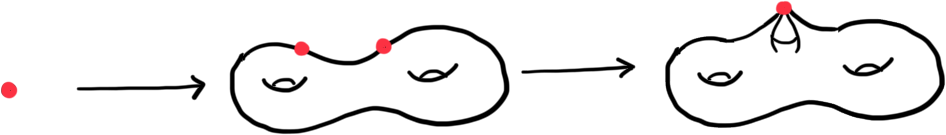
\includegraphics[width=0.7\textwidth]{images/Sketch.png}
    \end{center}
\end{example}

It can be shown that every singular complex projective variety \(X\) admits a
mixed Hodge structure, although we do not prove it. We can then use this Hodge
structure to define the \textit{generalised intermediate Jacobians}
\[
    \IJac^k X = \frac{\HH^{2k+1}(X,\mathbb{C})}{F^k
    H^{2k-1}(X,\mathbb{C})+\HH^k(X,\mathbb{Z})},
\]
for \(k\geq 1\). As before we say \(\text{IJac}^1=\text{Jac}\) is the (generalised) Jacobian.

Note the subgroup by which we quotient is no longer a direct sum! Consequently,
the intermediate Jacobian is not always an Abelian variety. It is, however,
always an extension of an Abelian variety by an algebraic torus
\((\mathbb{C}^\times)^b\). Such objects are called \textit{semi-Abelian
varieties}.

For instance \(X\) is an irreducible curve with one node and \(\tilde X\) is its
normalisation, our computation shows there is an exact sequence
\[
    0\to \mathbb{C}^\ast\to \Jac X \to \Jac \tilde X\to 0.
\]
Given such a curve \(X\) we can consider a smoothing (i.e.\ a family of curves
with unique non-singular fiber \(X\)) and chase through a diagram to show a
Mumford--Newstead type result, that \(\Jac X\) coincides with the second
intermediate Jacobian of a moduli space of rank \(2\) bundles with fixed
determinant. Combined with Namikawa's result, we then have the following.

\begin{theorem}[(Basu--Dan--Kaur)]
    Let \(X_0, X_1\) be irreducible nodal curves of genus \(g\geq 4\) with
    exactly one node, such that the normalizations \(\tilde{X}_0\) and
    \(\tilde{X_1}\) are not hyper-elliptic. Let \(L_0\) and \(L_1\) be
    invertible sheaves of odd degree on \(X_0\) and \(X_1\), respectively. Then
    \(X_0\cong X_2\) if and only if \(\Moduli_{2,L_0}X_0\cong
    \Moduli_{2,L_1}X_1\), where  \(\Moduli_{2,L_0}(X_0)\) denotes the Gieseker
    moduli space of rank \(2\) vector bundles with determinant \(L_0\) on
    curves semi-stably equivalent to \(X_0\).
\end{theorem}
